\chapter*{Conclusion}
	\thispagestyle{conclusion}
	\addcontentsline{toc}{chapter}{Conclusion}
	
	
Grâce à son utilisation de problèmes SMT, des tests comme spécifications et sa vision de la méthode défaillante comme une boîte noire, OLS-Repair permet de répondre brillamment à la question initiale : Est-il possible de réparer des programmes tout en étant indépendant des bugs présents ? Cette approche pourrait également être utilisée lors d'un développement en TDD\footnote{\url{https://fr.wikipedia.org/wiki/Test_driven_development}} dans le but d'écrire uniquement les tests et de synthétiser le comportement voulu plutôt que de l'écrire. 
\par OLS-Repair est encore jeune et il existe de nombreux axes d'améliorations :  
la collecte des données pourrait être dynamique afin de récuperer plus d'informations comme par exemple, les valeurs des attributs de classes lors de l'exécution d'un test. 
La détection de la méthode défaillante pourrait se baser sur	 les stacktraces des différents tests.
Il est aussi possible d'augmenter le nombre de types de données supportés dans les spécifications. 
Une idée originale serait également d'étendre le principe des méthodes comme boîte noire à des fragments de codes. Pour finir, on pourrait imaginer l'intégration de cette approche dans des outils tels que Nopol\cite{nopol} puisque le comportement est sensiblement identique.


\begin{center}
	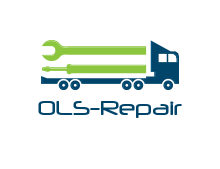
\includegraphics[scale=1]{OLS-logo.png}
\end{center}
	
	

